
\chapter{Framework in Theory}\label{chapter:Foundation}
In this chapter we explain the framework model in theory, the key concepts behind it, challenges facing the design and their possible solutions.


\section{Foundation}
	The fundamental core element of this framework is the computational unit derived from the use case. One possible abstraction of the computational unit is the \textit{flow}, which is a purposeful unit of computation that contains groups of sequential instructions "\textit{elements}" whose input/output are connected together. These elements could have a significant meaning on their own such as snapping a photo or making simple data transformation as shown in figure \ref{fig:flow}. Also, A flow can not only be a standalone self-contained computation, but can interact with other flows in which they collaborate for data gathering, sharing and processing as well.
	
	
\begin{figure}[H]
	\centering
	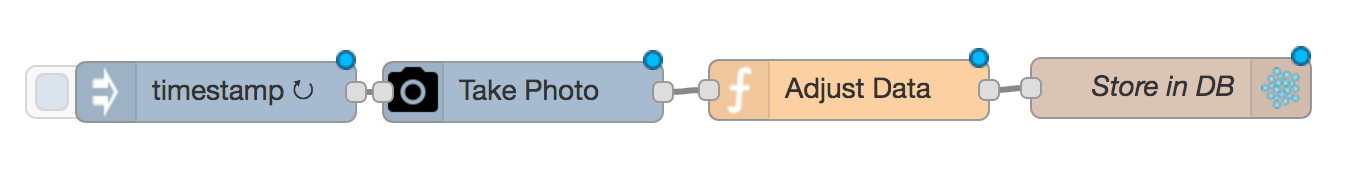
\includegraphics[scale=0.5]{images/db-out.png} 
	\caption{A node-red flow that stores an image in a database every time interval}
	\label{fig:flow}
\end{figure}

After having defined flows, the next step is ti execute them. To begin with, we must address the challenge that flows are distributed in the sense that each flow could reside on a different node. In addition, as previously mentioned, flows may interact, therefore, they need a way to communicate. Moreover, since nodes might be disconnected,  the communication mechanism must not require end-to-end paths. Furthermore, it  should handle sending the computations themselves from one node to another, at the end we are designing a pervasive framework that should manage sending computations everywhere.\\

\noindent Another challenge that faces the execution of  flows, are the dependencies and resources needed to carry out the execution.
 They might vary from one use case to another, thus need to be orchestrated across nodes though the messaging system by  ensuring the delivery of relevant dependencies along with their respective computations.\\
 
\noindent Now assuming that we can send flows to the nodes, make them communicate and satisfy their dependencies and provide their resources, one aspect remains, which is triggering the execution of flows. There are multiple ways to start an execution, one simple example is a time interval trigger. Other ways include starting the execution when new data has been received or other events have been triggered e.g. via physical sensors.\\


\noindent A flow should be modular having a specific functionality with defined interfaces that reduce the complexity, allowing re-use and re-assembly. Moreover, since flows should be composable, they need to interact and exchange data. Think of composability as LEGO parts that need to be assembled in their correct positions in order to create a figure, however in contrast to individual LEGO parts which do not have a meaning on their own, individual flow elements could serve a specific purpose besides their global one. \\
 
\noindent  To establish flow composability in our context, we need to be able to match the output data of one flow to the input data of another, no matter whether the flows are on the same node or distributed; connected or disconnected. For instance in general terms, if we have a flow \(f_1\) that takes \(A\) as input and gives \(B\) as an output
\[ f_1 : A  \to B  \]
and another flow \(f_2\) that takes \(B\) as an input and gives a new output \(C\)
% the output of \(f_1\) and produce a new result and so on. 
\[ f_2 : B  \to C  \]
we should be able to compose a new flow by taking \(f_1\)'s output and giving \(f_2\)'s input, resulting in flow \(f_3\) which is a composite of both:
\[f_3: A \to C = f_2 \circ f_1 .\]

 \noindent Composability ensures that regardless the use case, logic or implementation of a flow, it still can be composable if it matched the input/output of another flow. Composability should be valid in both local and distributed environments. Thus, in the case of local flow composability, there should be a way to connect the output of a flow to the input of another locally as shown in \ref{fig:compose}. In the case of distributed composability, the messaging system should connect the flows and serve as a broker to deliver the data as shown in \ref{fig:compose2}. 

\begin{figure}[H]
	\centering
	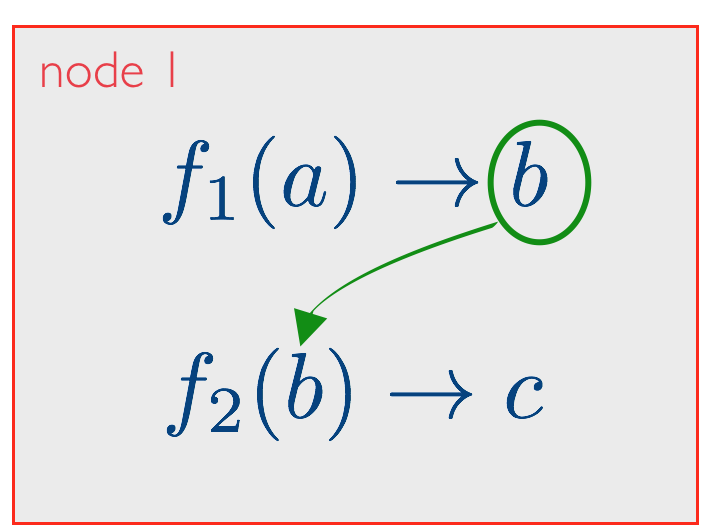
\includegraphics[scale=0.5]{images/local-compose.png} 
 	\caption{A node containing two composable flows}
	\label{fig:compose}
\end{figure}
\begin{figure}[H]
	\centering
	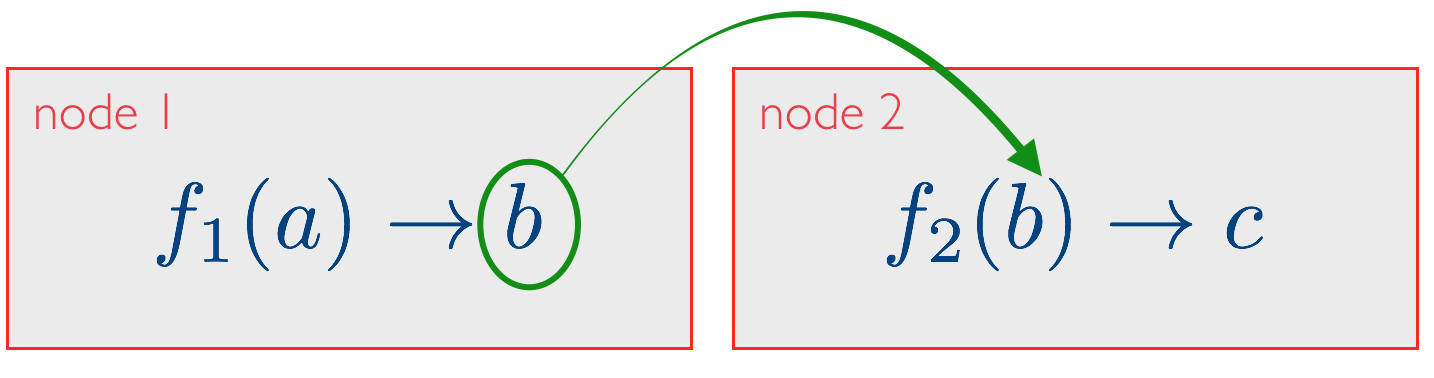
\includegraphics[scale=0.5]{images/distributed-compose.png}
	\caption{Two separate nodes having distributed composability}
	\label{fig:compose2}
\end{figure}

\noindent To sum up, flows are distributed and modular units of computation derived from a use case which require dependencies and resources. They communicate with each other and can be composed both locally and in a distributed manner. By achieving  modularity and composability, flows can be assembled in different combinations, thus allowing re-use and extensibility.
\newpage
\section{Computational Model}

Below we present the computational model as an abstraction for the framework design. It explains the components, challenges and the possible solutions that could be implemented to overcome these challenges. 	

\subsection{Distributed Nodes \& Flows}
In order to start with the framework explanation we must understand the idea behind pervasiveness. Pervasive computing relies on the idea of pushing flows to the edge "nodes" and thus it is fundamentally distributed. A system is distributed if its components  are on networked computers which communicate only by sending and receiving of messages \cite{DSYS} which is the case here. Now in our model, each node should be capable of executing flows and producing results as long as it has the required dependencies and resources. Moreover, to ensure that flows are composable, nodes should be able to communicate seamlessly even though nodes hosting this flows might be disconnected. Moreover, the model should be delay tolerant and subject to connection failures.\\



\noindent Turning to flows, in essence every challenge related to making the nodes distributed also applies to flows because nodes host flows. However, there are more to flows, distributing them across nodes could have different approaches depending on the use case. Let us explain this with figure \ref{fig:distributing-flows}, to start with, lets take the set of all nodes in the system and call it \(S(t)\) which is a function of time since nodes can be removed or added to the system dynamically at any instant of time. Moreover, nodes in  Then comes the candidate set \(S_C(t)\), which are nodes that satisfy the required dependencies and resources of a certain computation. Note that, nodes inside any of the these sets might not have end-to-end path. Given \(S_C(t)\), the flows could be either sent to a random set of nodes or to a specific set of nodes. This provides flexibility in applying the use case without wasting resources. In addition, it magnifies the effect of locational context, meaning that if we want to compute a certain computation or measurement in a specific location  and we know the general identifiers of  the  nodes residing in this location, we can send a flow to this exact set of nodes with our desired computation. Continuing to explain flows approaches with figure \ref{fig:distributing-flows}, a flow could be distributed across nodes of the candidate set  \(S_C(t)\) in multiple ways explained as follows: (i) flows are sent to all nodes in  \(S_C(t)\), (ii) flows are sent to a set of  \(n\)  nodes where \(n > 1\), whether they are selected as case \textit{C \#2} in the figure or picked at random, (iii) choosing only one node to execute a specific flow \textit{C \#1}. As a result, the communication model is one of the most crucial parts to guarantee a distributed system, it should have the flexibility to provide these approaches and overcome the hurdle of disconnected nodes.
 
 \begin{figure}[H]
 	\centering
 	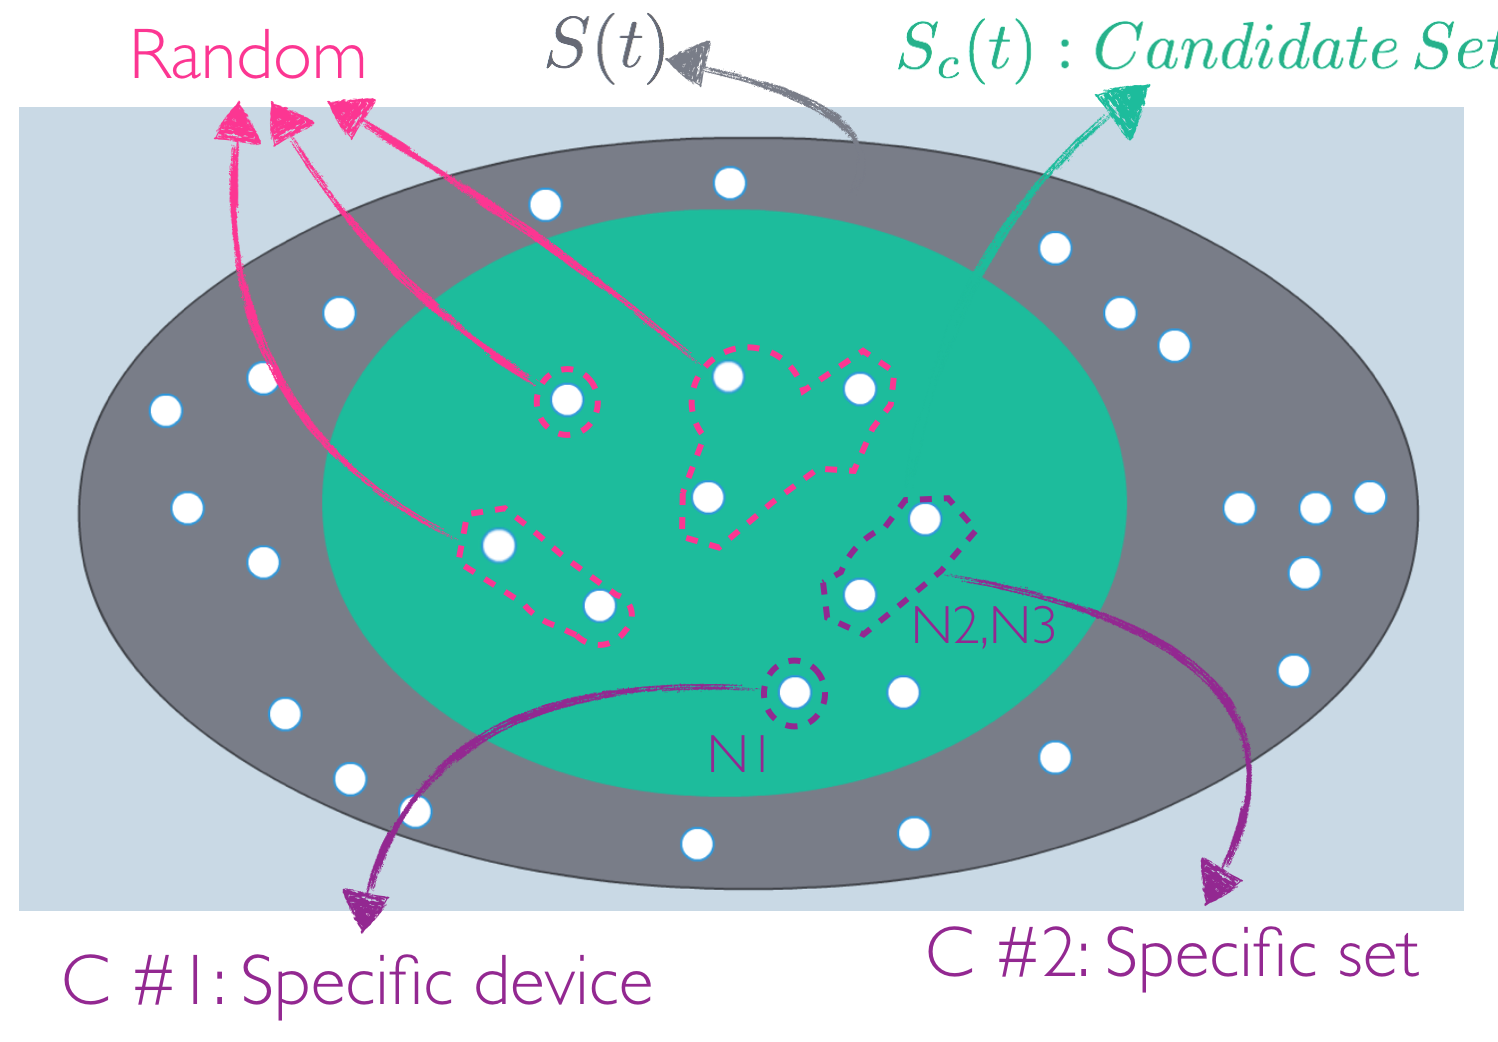
\includegraphics[scale=0.45]{images/set.png} 
 	\caption{Distributing flows approaches}
 	\label{fig:distributing-flows}
 \end{figure}

\noindent Another main challenge is to actually find the connected nodes. Distributed and pervasive environments are dynamic, their components are not known to be live or dead at compile-time. Thus the framework should be able to run service discovery at run-time in order to find the connected nodes or it should be able to broadcast its message to all the other nodes and receive them as well. Otherwise, the approach would not qualify to be a distributed system. \\

\noindent There are possible ways to achieve that, one could set up a static DNS server to resolve the domain name of a node, however, this requires having static IP's for all the nodes. Another solution is to use DDNS or MDNS to update the domain name whenever an ip changes dynamically.









\subsection{Software Dependencies}

Dependencies are one of the main requirements of computation execution, dropping one or more dependencies would stop the execution from proceeding. Thus, we need to deal with them and make sure that all dependencies are satisfied.  There are two types of dependencies; the static software frameworks that the whole design relies on and must exist on each node, and the dynamic dependencies that are specific to each computation. \\

\noindent First, are the static dependencies are mainly the common libraries and software that most of the computations would require, they represent the base of framework. That is why these dependencies are installed to each node in our design, examples of these dependencies include the operating system, data store and any other standard or custom libraries that are used by most computations. In addition to, the messaging system which implements the communication model allowing interaction between nodes. \\

\noindent Second, are the dynamic dependencies which are specific to each computation such as additional scripts, configuration files or libraries. In this case, they cannot be installed at node initialization since we can not know what are the custom dependencies any computation would need beforehand. Therefore, the computational model design should allow a way to configure additional dependencies. Moreover, the communication mechanism should support this configuration and grant a way to carry the configured dependencies forward to other nodes.\\
 
 
\noindent Static dependencies create ambiguity. Suppose that we want to upgrade the versions of current libraries installed on the nodes. This introduces a  versioning problem, imagine that there is a computation on the node that uses an older version of the same library while the maintainer is upgrading to a newer version of the same library that is not backward compatible.  \\
  
\noindent Nevertheless, there are multiple possible solutions to remove the ambiguity and make  version upgrading more concrete; one solution would be to give the dependencies different names according to their versions before shipping them, hence, any different version would not replace the existing ones. Another solution would be to design a system that links each running computation on the node to its dependencies and once a collision appears, the new computation renames its dependency and uses the renamed one.
 

\subsection {Resources " Physical Dependencies" }


Resources are physical dependencies which are also necessary for computations to run. However, they might differ or not exist at all on each node. If one of the needed resources is missing then the computation could be either dismissed or queued depending on the type of resource. Moreover, the maintainers cannot make any assumptions about the resources, meaning, an assumption stating that each node has a camera is not necessarily true. Since the resources are not standardized across all nodes, each computation must provide meta data expressing the resources it is going to require, also, the node must realize its available resources. Then a node can check against its capabilities and decide whether it could carry out the execution or not. Further, the meta data can be exposed to the routing layer, thus helping the router take an informed decision whether a specific route contains nodes with the required resources or not. This could also provide an insight for developing better routing algorithms.\\

 \noindent Considering that each computation model has meta data describing its resource consumption, then it is possible to know if it is going to be deployed on a specific node or not. Additionally, if it is not going to be deployed then it should be decided whether the computation is going to be queued or dismissed according to the possibility of acquiring the resource. The idea of queuing computations however develops a scheduling problem. Since we have a queue of computations inside each node, we will have a race condition on which computation should be deployed first according to available resources. Furthermore, since some computations might be dismissed, a rather bigger scheduling problem will come up when we try to fit the all computations across nodes in the whole system framework.\\

  \noindent There are two types of resources; sensors and actuators which are used throughout a computation, and the hardware resources which influences the performance requirements of a specific computation.


\subsubsection{Sensors and Actuators}

  Sensors and actuators are resources attached to a node such as cameras, temperature and gas sensors. Executing a computation missing this type of resource on a node should have a lower possibility of being queued, since its highly unlikely that this resource would be attached soon. However sensors and actuators are dynamic, they can be added or removed on demand, therefore, having them in a specification file as a static dependency which is only set at initialization time will be troublesome. Of course, we can always edit the specification file once we change the state of any of these resources, but this solution is not very efficient nor scalable, as it increases the manual work. It would be much easier if the node could run resource discovery to find its attached resources each time it receives a computation. \\
  
  \noindent Moving on to consider computations acquiring the same resource at the same time, for instance, two computations that want to take a photo at the same time. This is problematic because whichever computation acquires a lock on the camera first will succeed while the other will fail. Therefore as a resolution, we could use resource decoupling; instead of having the computation ask a specific resource directly for information, the  data will be pushed into a database. Afterwards, the different computations could query the data from a database.
  
  

\subsubsection{Hardware Resources }

The second type of resources is related to the node performance, its power and memory capabilities, it is heavily biased by the  node processor  and its random access memory type and size. Computations vary in terms of resource consumption and hence a heavy computation should not be deployed to a node which is already loaded. \\

\noindent Queuing this type of dependencies should have a higher probability because it is highly possible that one of the computations will finish soon, thus decreasing the cpu usage and freeing more memory.







\subsection{Pub-Sub Messaging Queues}\label{subsec:pub-sub}

The communication model is an essential part of this framework, it solves some of the biggest challenges, which are in a nutshell, service discovery, carrying dependencies, sending and receiving of data or computations whether nodes have  end-to-end paths or not. Moreover, given our distributed approach and the need for service discovery, the communications model cannot be  end-point centric since in the general case we are unable to target the actual nodes with their host names as endpoints. The reason for that is, we do not know their respective addresses or either they are connected or not. Rather our communication model is data-centric or information-centric meaning it assumes that there are some parties interested in sending data and others willing to receive the same data given a certain context and regardless their network location. \\

 

\noindent A possible solution to the framework demands and challenges is to use publish-subscribe message queues. The pub-sub pattern is data centric messaging architecture in which senders also known as \textit{publishers} do not send messages directly to receivers, rather send to specific topics. Then, \textit{subscribers} receive messages which are relevant to them by subscribing to these topics. \\


\noindent Commonly the pub-sub message queues contains a centralized bus \textit{broker} which handles publishing, subscribing, notifying and persistence. 
When the bus receives a message published on a specific topic, the data is stored on a local storage for persistence and failure recovery. 
Parties can subscribe to the data topics on the  bus hence notified when a new message is published. Figure \ref{fig:message-queues} shows  publishers publishing data to topic \textit{t1} on the bus, subscribers subscribing to \textit{t1} and notified when a new message is on the bus.
	
\begin{figure}[H]
	\centering
	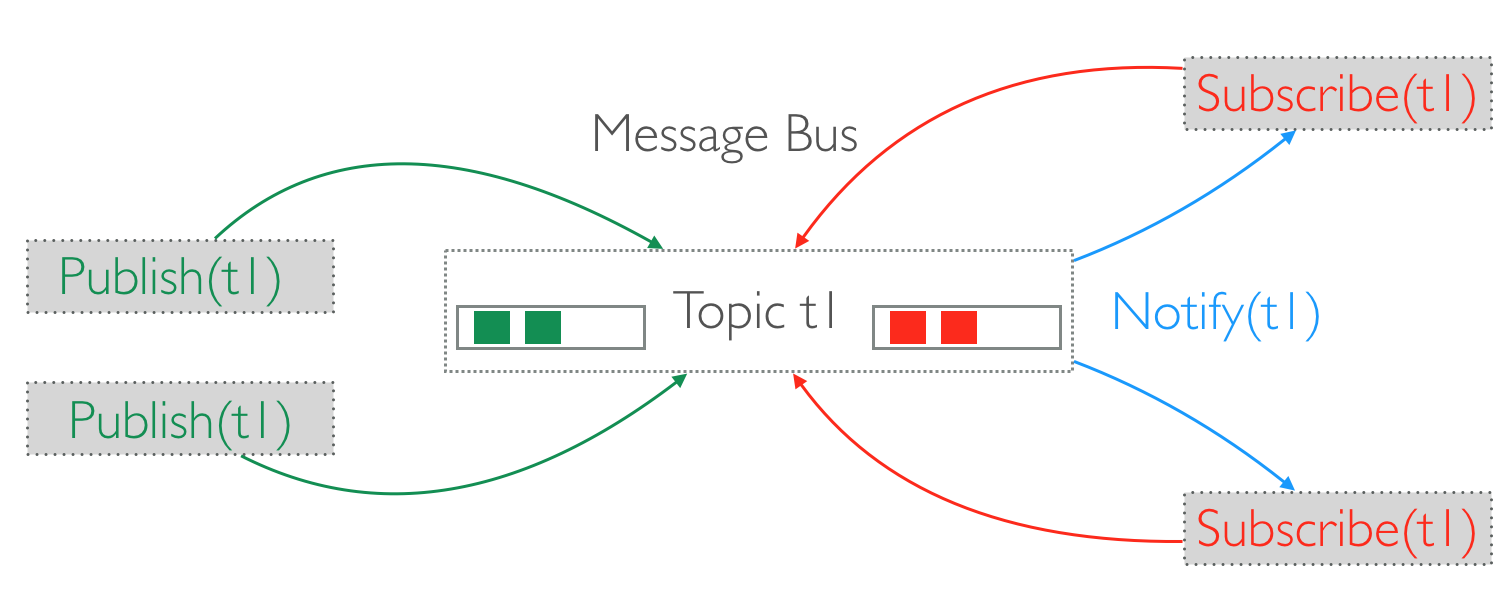
\includegraphics[scale=0.3]{images/message-queues.png}
	\caption{Common message queues}
	\label{fig:message-queues}
\end{figure}

\noindent However having a pub-sub message queue with a centralized bus can not be used in our case. Since we do not know machines addresses or host names thus knowing where is the centralized message queue located is not possible. Therefore, each party or node would have its own message bus and local storage which are then synchronized together whenever there is a connection.

\begin{figure}[H]
	\centering
	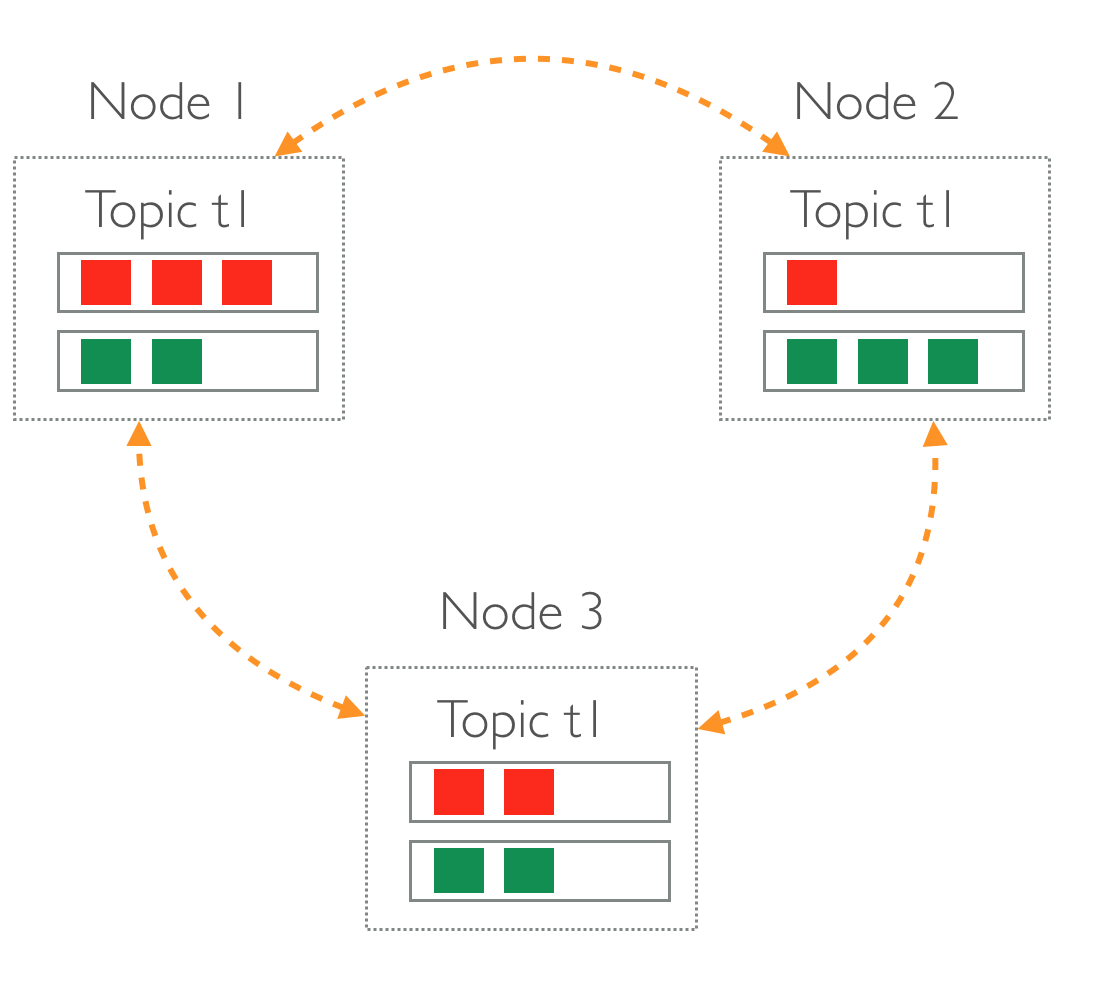
\includegraphics[scale=0.3]{images/de-message-queues.png}
	\caption{De-centralized message queues}
	\label{fig:de-message-queues}
\end{figure}
 Now addressing the mentioned challenges:

\begin{itemize}
\item First off, nodes service discovery, messaging queues are able to discover and synchronize messages across all the nodes connected to the messaging system through any kind of network.  They are also dynamic in the sense that they are sensitive to the addition or removal of new nodes to or from the system. 

\item  Having solved the problem of service discovery, nodes can now send and receive messages. But since we also care to send computations as well, we must differentiate between data  and computations messages. Thus, a possible solution is to reserve a unique topic only for exchanging computations between nodes.

\item For sending data or computation messages to a random set of  \(n\) nodes, a routing algorithm can be used to ensure that no more than \(n\) nodes will receive the message. Further, if we exposed the meta data of the computation, the routing algorithm can make sure that receiving nodes will have a higher probability of being able to execute the flow.

\item Sending data or computation messages to specific node or set of nodes can be done by reserving a unique topic for each. Therefore, to target any node, the message should be published once to each unique topic. For example, if we use the general identifier as a unique topic and want to publish a message to node 1, then, we can create  unique topic \textit{"N \#1 "} and send the messages over this topic.

 
\item Pub-sub messaging queues allow carrying arbitrary kinds of data inside the message body. Therefore, computation dependencies can be  added to the message body of their respective computations. Thus solving the obstacle of carrying dependencies mentioned earlier and creating self-contained computations that are ready to execute anywhere.

\item Last but not least, in order to send data or computation messages to disconnected nodes, either because there exists no end-to-end path or the nodes are experiencing network connectivity issues. The pub-sub messaging system should be delay tolerant and implements the store-carry-forward technique, this will allow the messaging system to store messages until connectivity is back or keep the message hopping from one device to another till it finds its end destination.
\end{itemize}

\noindent Having found a solution for our communication model challenges assists us to focus on the framework design and implementation. Knowing that the underlying network model will not fail us to connect the nodes even without and end-to-end path. In addition, we can directly send and receive message to the nodes on data topics without the framework being aware of their host names or network addresses.  




\section{Data Model}
In this section we describe the data model which includes the structure of the data sent between nodes through the messaging system, how the data travels from one node to another and the input/output specification used to combine and compose different flows.

\subsection{Data Types}
A computational flow can generate different types of data depending on the use case. This data could be intermediate processing data or a computational result. Also, we should not attempt restrict the data types in order to make sure the framework is as dynamic as possible. The challenge is to be able to represent these data types in a composable way. Therefore, if a developer wants to create a composable flow he/she should define an IO specification explained latter. However, the good thing is that, the developer dictates how the input or output data are structured while developing the computational flow. Hence, he/she is in complete control and can structure the data in any way as long as it can be used afterwards.  Different data types include: i) structured data that could be stored either in a relational or non-relational data base, ii) unstructured data, iii)  data streams.

\subsection{Moving Data}

Moving data is the idea  to send/receive raw or processed data to any flow. We should be to able use data from different remote or local sources in any computation. Some use cases for moving data are:
\begin{itemize}
\item Composing flows is one of the main use cases, we would like to get input data for a computation from the output of another.

\item We can send data to be processed by a computational flow on any node and then obtain the outcome. For instance, we can send an image to a node containing computational flow with image recognition algorithm, then the image gets processed on that node and we get back the computation results. 

\item A Node can act as a monitoring node in which it is interested in all outputs of a certain computation running on several nodes.

\end{itemize} 
 As mentioned in \ref{subsec:pub-sub}, our approach and communication model is data-centric. Therefore, flows could subscribe/publish to a certain data topic in the distributed pub-sub messaging queue. Thus, data should reach any node which contains a flow subscribed to a certain topic. This allows us to move data freely and at will, we just need to express how a flow receives or publishes data.

\subsection{IO Specification}
Turning now to consider the input and output specification, the IO spec. explains how the output of a flow in one node can be linked to the input of another flow either on the same node or on a remote one. There are multiple ways to specify how the IO data communicates which are explained below:


\begin{itemize}
	\item The first way allows data communication between computations of the same node  through a database. One computation writes interesting data into a specific table with locally unique name in a database. Then, any other local computation which wants to use this data is allowed to fetch it from this table. Unique names are suggested to decrease the possibility of database inconsistencies if someone is using a table with the same name.
	 
	Flows can be used to describe the database configuration from inside the computation flow, thus the maintainer should make sure when developing  locally composable flows that the database configuration and table names match. An example in figure \ref{fig:db} shows that the first flow takes an image and then store it in the database with a unique table name.  While the second flow, pulls the data from the database upon receiving a request on a specific URL. 
	
	\begin{figure}[H]
		\centering
		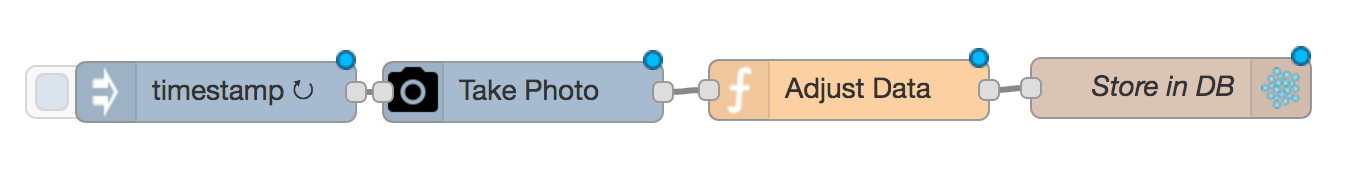
\includegraphics[scale=0.5]{images/db-out.png}
		
\includegraphics[scale=0.5]{images/db-in.png}
		\caption{Two separate computational flows describing the IO through a database.}
		\label{fig:db}
	\end{figure}
	
	\item Another way is to use  publish-subscribe messaging pattern to communicate through different nodes. The node which generates the data publishes its resulting data to a generally unique topic, therefore any node interested in the data could simply subscribe to that topic and process the data accordingly.
	
Figure \ref{fig:scampi} shows two flows as an example of this method, the first flow generates data and publishes it to the messaging system. Then, on any node, the data could be received via subscribing to the same topic.
	
	\begin{figure}[H]
		\centering
		
\includegraphics[scale=0.6]{images/SCAMPI-pub.png}
		
\includegraphics[scale=0.6]{images/SCAMPI-sub.png}
		\caption{Two composable flows exchanging data via the messaging system.}
		\label{fig:scampi}
	\end{figure}
	
	\item Streaming data is also possible, one node can have a computation serving as a streaming server while other nodes have computations which act as clients. However, the global reference of the streaming server must be known to clients or to make it more dynamic, a service discovery mechanism could be implemented in order to help clients find streaming servers.
\end{itemize}	


\section{Summary}

To conclude this chapter, we explained the key concepts and foundations behind this framework, what is a flow and how it can be composed. We also described the computational model as an abstraction the framework design, and illustrated the challenges that faces this model which included  dealing with dependencies, resources and having a distributed system model in addition to their possible solutions . We also elaborated the communication model and how it solves some of the challenges in our design. Moreover, we have shown how data inside the computation can be structured, and how input and output data of different nodes could be connected together.


